\chapter{\luDecompTitle}
\label{LUdecomp}

Certain matrices are easier to work with than others.  In this section, we will see how to write any square\footnote{The case where $M$ is not square is dealt with at the end of the lecture.} matrix $M$ as the product of two simpler matrices.  We will write $$M=LU\, ,$$ where:
\begin{itemize}
\item $L$ is \emph{lower triangular}\index{Lower triangular matrix}.  This means that all entries above the main diagonal are zero.  In notation,
$L=(l^i_j)$ with $l^i_j=0$ for all $j>i$.
\[L=\begin{pmatrix}
l^1_1 & 0 & 0 & \cdots \\
l^2_1 & l^2_2 & 0 & \cdots \\
l^3_1 & l^3_2 & l^3_3 & \cdots \\
\vdots & \vdots & \vdots & \ddots \\
\end{pmatrix}
\]

\item $U$ is \emph{upper triangular}\index{Upper triangular matrix}.  This means that all entries below the main diagonal are zero.  In notation,
$U=(u^i_j)$ with $u^i_j=0$ for all $j<i$.
\[U=\begin{pmatrix}
u^1_1 & u^1_2 & u^1_3 & \cdots \\
0 & u^2_2 & u^2_3 & \cdots \\
0 & 0 & u^3_3 & \cdots \\
\vdots & \vdots & \vdots & \ddots \\
\end{pmatrix}
\]
\end{itemize}
$M=LU$ is called an \emph{$LU$ decomposition}\index{LU@$LU$ decomposition} of $M$.

This is a useful trick for  computational reasons; it is much easier to compute the inverse of an upper or lower triangular matrix than general matrices.  Since inverses are useful for solving linear systems, this makes solving any linear system associated to the matrix much faster as well.  The determinant---a very important quantity associated with any square matrix---is very easy to compute for triangular matrices.

\begin{example}
Linear systems associated to upper triangular matrices are very easy to solve by back substitution.
\[
\begin{amatrix}{2}
a & b & 1 \\
0 & c & e \\
\end{amatrix} \ \Rightarrow \ y=\frac{e}{c}\, , \quad x=\frac{1}{a}\left(1-\frac{be}{c}\right)
\]

\[
\begin{amatrix}{3}
1 & 0 & 0 & d \\
a & 1 & 0 & e \\
b & c & 1 & f \\
\end{amatrix} \Rightarrow x=d\, , \qquad y=e-ad\, , \qquad z=f-bd-c(e-ad)
\]
For lower triangular matrices, \emph{back} substitution\index{Back substitution} gives a quick solution; for upper triangular matrices, \emph{forward} substitution\index{Forward substitution} gives the solution.
\end{example}





\section{Using $LU$ Decomposition to Solve Linear Systems}

Suppose we have $M=LU$ and want to solve the system
\[
MX=LUX=V.
\]

\begin{itemize}
\item{Step 1:} Set $W=\colvec{u\\v\\w}=UX$.  

\item{Step 2:} Solve the system $LW=V$.  This should be simple by forward substitution since $L$ is lower triangular.  Suppose the solution to $LW=V$ is $W_0$.  

\item{Step 3:} Now solve the system $UX=W_0$.  This should be easy by backward substitution, since $U$ is upper triangular.  The solution to this system is the solution to the original system.
\end{itemize}
We can think of this as using the matrix $L$ to perform row operations on the matrix $U$ in order to solve the system; this idea also appears in the  study of determinants.

%\href{\webworkurl ReadingHomework11/1/}{Reading homework: problem 11.1}
\reading{11}{1}

\begin{example}
Consider the linear system:
\[
      \begin{linsys}{4}
            6x & +&18y & +&3z         &=& 3  \\[1mm]
            2x & +&12y & +&z	    &=& 19 \\[1mm]
            4x & +&15y & +&3z         &=& 0  
      \end{linsys}
\]

An $LU$ decomposition for the associated matrix $M$ is:
\[
\begin{pmatrix}
6 & 18 & 3 \\
2 & 12 & 1 \\
4 & 15 & 3 
\end{pmatrix} =
\begin{pmatrix}
3 & 0 & 0 \\
1 & 6 & 0 \\
2 & 3 & 1 
\end{pmatrix}
\begin{pmatrix}
2 & 6 & 1 \\
0 & 1 & 0 \\
0 & 0 & 1 
\end{pmatrix}.
\]

\begin{itemize}
\item{Step 1:} \hypertarget{LUproc}{Set} $W=\colvec{u\\v\\w}=UX$.  

\item{Step 2:} Solve the system $LW=V$:

\[
\begin{pmatrix}
3 & 0 & 0 \\
1 & 6 & 0 \\
2 & 3 & 1 
\end{pmatrix}
\colvec{u\\v\\w} =
\colvec{3\\19\\0}
\]

By substitution, we get $u=1$, $v=3$, and $w=-11$.  Then 
\[W_0=\colvec{1\\3\\-11}\]

\item{Step 3:} Solve the system $UX=W_0$.  
\[
\begin{pmatrix}
2 & 6 & 1 \\
0 & 1 & 0 \\
0 & 0 & 1 
\end{pmatrix}
\colvec{x\\y\\z} =
\colvec{1\\3\\-11}
\]
Back substitution gives $z=-11, y=3$, and $x=-3$.  

Then $X=\colvec{-3\\3\\-11}$, and we're done.
\end{itemize}
\end{example}

\videoscriptlink{lu_decomposition_using_lu_decomp.mp4}{Using a $LU$ decomposition}{scripts_lu_decomposition_using_lu_example}

%\begin{figure}
\begin{center}
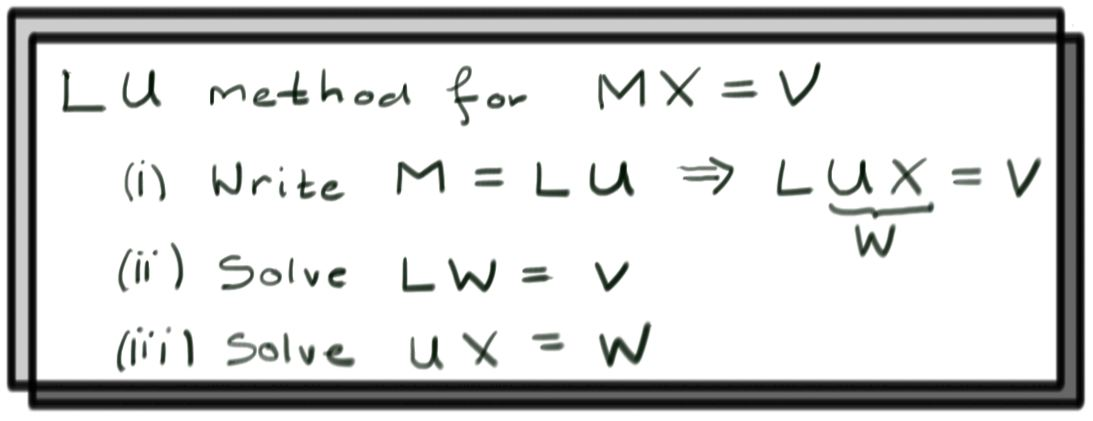
\includegraphics[scale=.3]{\luDecompPath/LU_solution.jpg}
\end{center}
%\end{figure}

\section{Finding an $LU$ Decomposition.}
\label{finding_LU_decomp}
 
For any given matrix, there are actually many different $LU$ decompositions.  However, there is a unique $LU$ decomposition in which the $L$ matrix has ones on the diagonal. In that case $L$ is called a \emph{lower unit triangular matrix}\index{Lower unit triangular matrix}.

To find the $LU$ decomposition, we'll create two sequences of matrices $L_0, L_1, \ldots$ and $U_0, U_1, \ldots$ such that at each step, $L_iU_i=M$.  Each of the $L_i$ will be lower triangular, but only the last $U_i$ will be upper triangular.

Start by setting $L_0=I$ and $U_0=M$, because $L_0U_0=M$. A main concept of this calculation is captured by the following example:

\begin{example}
Consider $$E=\begin{pmatrix}1&0\\\lambda&1\end{pmatrix}\, ,\qquad M=\begin{pmatrix}a&b&c&\cdots\\d&e&f&\cdots\end{pmatrix}\, .$$
Lets compute $EM$
$$
EM=\begin{pmatrix}a&b&c&\cdots\\d+\lambda a&e+\lambda b&f+\lambda c&\cdots\end{pmatrix}\, ,.
$$
Something neat happened here: multiplying $M$ by $E$ performed the row operation $R_2\to R_2+\lambda R-1$ on $M$.
Another interesting fact:
$$
E^{-1}:=\begin{pmatrix}1&0\\-\lambda&1\end{pmatrix}
$$ 
obeys (check this yourself...)
$$
E^{-1} E = 1\, .
$$
Hence $M=E^{-1} E M$ or, writing this out
$$
\begin{pmatrix}a&b&c&\cdots\\d&e&f&\cdots\end{pmatrix}=\begin{pmatrix}1&0\\-\lambda&1\end{pmatrix} \begin{pmatrix}a&b&c&\cdots\\d+\lambda a&e+\lambda b&f+\lambda c&\cdots\end{pmatrix}\, .
$$
Here the matrix on the left is lower triangular, while the matrix on the right has had a row operation performed on it.
\end{example}




\vspace{2mm}
We would like to  use the first row of $U_0$ to zero out the first entry of every row below it.  For our running example, $$U_0=M=\begin{pmatrix}
6 & 18 & 3 \\
2 & 12 & 1 \\
4 & 15 & 3 
\end{pmatrix}\, ,$$ so we would like to perform the row operations $R_2\to R_2 -\frac 13 R_1$ and $R_3\to R_3-\frac 23R_1$.
%so the second row minus $\frac{1}{3}$ of the first row will zero out the first entry in the second row.  Likewise, the third row minus $\frac{2}{3}$ of the first row will zero out the first entry in the third row.
If we perform these row operations on $U_0$ to produce 
$$U_1=\begin{pmatrix}
6 & 18 & 3 \\
0 & 6 & 0 \\
0 & 3 & 1 
\end{pmatrix}\, ,$$
we need to multiply this on the left by a lower triangular matrix $L_1$ so that the product $L_1U_1=M$ still.
The above example shows how to do this:
Set $L_1$ to be the lower triangular matrix whose first column is filled with the minus constants used to zero out the first column of $M$.  Then $$L_1 = \begin{pmatrix}
1 & 0 & 0 \\[1mm]
\frac{1}{3} & 1 & 0 \\[1mm]
\frac{2}{3} & 0 & 1 
\end{pmatrix}\, .$$  
%Set $U_1$ to be the matrix obtained by zeroing out the first column of $M$.  Then $U_1=\begin{pmatrix}
%6 & 18 & 3 \\
%0 & 6 & 0 \\
%0 & 3 & 1 
%\end{pmatrix}$.
By construction $L_1 U_1=M$, but you should compute this yourself as a double check.

Now repeat the process by zeroing the second column of $U_1$ below the diagonal using the second row of $U_1$ using the row operation
$R_3\to R_3-\frac 12 R_2$ to produce
$$U_2=\begin{pmatrix}6&18&3\\0&6&0\\0&0&1\end{pmatrix}\, .$$
The matrix that undoes this row operation is obtained in the same way we found $L_1$ above and is:
$$
\begin{pmatrix}
1&0&0\\
0&1&0\\
0&\frac 12& 0
\end{pmatrix}\, .
$$
Thus our answer for $L_2$ is the product of this matrix with $L_1$, namely
$$
L_2=
\begin{pmatrix}
1 & 0 & 0 \\[1mm]
\frac{1}{3} & 1 & 0 \\[1mm]
\frac{2}{3} & 0 & 1 
\end{pmatrix}\begin{pmatrix}
1&0&0\\
0&1&0\\
0&\frac 12& 0
\end{pmatrix}
=\begin{pmatrix}
1 & 0 & 0 \\[1mm]
\frac{1}{3} & 1 & 0 \\[1mm]
\frac{2}{3} & \frac{1}{2} & 1 
\end{pmatrix}\, .
$$
Notice that it is lower triangular because 

\begin{center}
\textcolor{brown}{THE PRODUCT OF LOWER TRIANGULAR MATRICES IS ALWAYS LOWER TRIANGULAR!}
\end{center}

\noindent
Moreover it is obtained by recording minus the constants used for all our row operations in the appropriate columns (this always works this way).
Moreover, $U_2$ is upper triangular and $M=L_2U_2$, we are done!
Putting this all together we have
$$M=\begin{pmatrix}
6 & 18 & 3 \\
2 & 12 & 1 \\
4 & 15 & 3 
\end{pmatrix}= \begin{pmatrix}
1 & 0 & 0 \\[1mm]
\frac{1}{3} & 1 & 0 \\[1mm]
\frac{2}{3} & \frac{1}{2} & 1 
\end{pmatrix}\begin{pmatrix}
6 & 18 & 3 \\
0 & 6 & 0 \\
0 & 0 & 1 
\end{pmatrix}\, .$$  
%Since $U_2$ is upper-triangular, we're done.  Inserting the new number into $L_1$ to get $L_2$ really is safe: the numbers in the first column don't affect the second column of $U_1$, since the first column of $U_1$ is already zeroed out.

If the matrix you're working with has more than three rows, just continue this process by zeroing out the next column below the diagonal, and repeat until there's nothing left to do.

\videoscriptlink{lu_decomposition_example.mp4}{Another $LU$ decomposition example}{scripts_lu_decomposition_example}

The fractions in the $L$ matrix are admittedly ugly.  For two matrices $LU$, we can multiply one entire column of $L$ by a constant $\lambda$ and divide the corresponding row of $U$ by the same constant without changing the product of the two matrices.  Then:

\begin{eqnarray*}
LU &=& \begin{pmatrix}
1 & 0 & 0 \\[1mm]
\frac{1}{3} & 1 & 0 \\[1mm]
\frac{2}{3} & \frac{1}{2} & 1 
\end{pmatrix}
I
\begin{pmatrix}
6 & 18 & 3 \\
0 & 6 & 0 \\
0 & 0 & 1 
\end{pmatrix} \\
&=&
\begin{pmatrix}
1 & 0 & 0 \\[1mm]
\frac{1}{3} & 1 & 0 \\[1mm]
\frac{2}{3} & \frac{1}{2} & 1 
\end{pmatrix}
\begin{pmatrix}
3 & 0 & 0 \\
0 & 6 & 0 \\
0 & 0 & 1 
\end{pmatrix}
\begin{pmatrix}
\frac{1}{3} & 0 & 0 \\[1mm]
0 & \frac{1}{6} & 0 \\[1mm]
0 & 0 & 1 
\end{pmatrix}
\begin{pmatrix}
6 & 18 & 3 \\
0 & 6 & 0 \\
0 & 0 & 1 
\end{pmatrix} \\
&=&
\begin{pmatrix}
3 & 0 & 0 \\
1 & 6 & 0 \\
2 & 3 & 1 
\end{pmatrix}\begin{pmatrix}
2 & 6 & 1 \\
0 & 1 & 0 \\
0 & 0 & 1 
\end{pmatrix}.
\end{eqnarray*}
The resulting matrix looks nicer, but isn't in standard (lower unit triangular matrix) form.

\reading{11}{2}
%\href{\webworkurl ReadingHomework11/2/}{Reading homework: problem 11.2}

For matrices that are not square, $LU$ decomposition still makes sense.  Given an $m\times n$ matrix $M$, for example we could write $M=LU$ with $L$ a square lower unit triangular matrix, and $U$ a rectangular matrix.  Then $L$ will be an $m\times m$ matrix, and $U$ will be an $m\times n$ matrix (of the same shape as $M$).  From here, the process is exactly the same as for a square matrix.  We create a sequence of matrices $L_i$ and $U_i$ that is eventually the $LU$ decomposition.  Again, we start with $L_0=I$ and $U_0=M$.

\begin{example}
Let's find the $LU$ decomposition of $M=U_0=\begin{pmatrix}
-2 & 1 & 3 \\
-4 & 4 & 1 
\end{pmatrix}$.  Since $M$ is a $2\times 3$ matrix, our decomposition will consist of a $2\times 2$ matrix and a $2\times 3$ matrix.  Then we start with $L_0=I_2=\begin{pmatrix}
1 & 0 \\
0 & 1
\end{pmatrix}$.

The next step is to zero-out the first column of $M$ below the diagonal.  There is only one row to cancel, then, and it can be removed by subtracting $2$ times the first row of $M$ to the second row of $M$.  Then:

\[
L_1=\begin{pmatrix}
1 & 0 \\
2 & 1
\end{pmatrix}, \qquad 
U_1 = \begin{pmatrix}
-2 & 1 & 3 \\
0 & 2 & -5 
\end{pmatrix}
\]
Since $U_1$ is upper triangular, we're done.  With a larger matrix, we would just continue the process.
\end{example}





\section{Block $LDU$ Decomposition}

Let $M$ be a square block matrix with square blocks $X,Y,Z,W$ such that $X^{-1}$ exists.  Then $M$ can be decomposed as a block $LDU$ decomposition, where $D$ is block diagonal, as follows:
\[
M=\begin{pmatrix}
X & Y \\
Z & W
\end{pmatrix}
\]

Then: \[M=\begin{pmatrix}
I &  0 \\
ZX^{-1} & I
\end{pmatrix}\begin{pmatrix}
X & 0 \\
0 & W-ZX^{-1}Y
\end{pmatrix}\begin{pmatrix}
I & X^{-1}Y \\
0 & I
\end{pmatrix}.\]
This can be checked explicitly simply by block-multiplying these three matrices.

\videoscriptlink{lu_decomposition_blocks.mp4}{Block $LDU$ Explanation}{scripts_lu_decomposition_blocks}

\begin{example}
For a $2\times 2$ matrix, we can regard each entry as a block.
\[
\begin{pmatrix}
1 & 2 \\
3 & 4
\end{pmatrix}=
\begin{pmatrix}
1 & 0 \\
3 & 1
\end{pmatrix}
\begin{pmatrix}
1 & 0 \\
0 & -2
\end{pmatrix}
\begin{pmatrix}
1 & 2 \\
0 & 1
\end{pmatrix}
\]
By multiplying the diagonal matrix by the upper triangular matrix, we get the standard $LU$ decomposition of the matrix.
\end{example}


%\section*{References}
%Wikipedia:
%\begin{itemize}
%\item \href{http://en.wikipedia.org/wiki/LU_decomposition}{$LU$ Decomposition}
%\item \href{http://en.wikipedia.org/wiki/Block_LU_decomposition}{Block $LU$ Decomposition}
%\end{itemize}

\section{Review Problems}



\begin{enumerate}

\item Let $D=\begin{pmatrix}
\lambda_1 & \mc0 \\
\mc0 & \lambda_2 \\
\end{pmatrix}$.
\begin{enumerate}
\item Write $D$ in terms of the vectors $e_1$ and $e_2$, and their transposes.
\item Suppose $P=\begin{pmatrix}
a & b \\
c & d \\
\end{pmatrix}$ is invertible.  Show that $D$ is similar to
\[
M=\frac{1}{ad-bc}\begin{pmatrix}
\lambda_1ad-\lambda_2bc & -(\lambda_1-\lambda_2)ab \\[1mm]
(\lambda_1-\lambda_2)cd & -\lambda_1bc + \lambda_2ad
\end{pmatrix}.
\]
\item Suppose the vectors $\rowvec{a,b}$ and $\rowvec{c,d}$ are orthogonal.  What can you say about $M$ in this case? (Hint: think about what \(M^T\) is equal to.)
\end{enumerate}

\phantomnewpage

\item \label{orthogprob} Suppose $S=\{v_1, \ldots, v_n \}$ is an \emph{orthogonal} (not orthonormal) basis for~$\Re^n$.  Then we can write any vector $v$ as $v=\sum_ic^iv_i$ for some constants $c^i$.  Find a formula for the constants $c^i$ in terms of $v$ and the vectors in~$S$.

\Videoscriptlink{orthonormal_bases_hint.mp4}{Hint}{scripts_orthonormal_bases_hint}
\phantomnewpage

\item \label{orthogprojprob} Let $u,v$ be linearly independent vectors in $\Re^3$, and $P=\spa \{ u,v\}$ be the plane spanned by $u$ and $v$.  
\begin{enumerate}
\item Is the vector $v^\bot := v-\frac{u\cdot v}{u\cdot u}u$ in the plane $P$?
\item  What is the (cosine of the) angle between $v^\bot$ and $u$?
\item %Given your solution to the above, 
How can you find a third vector perpendicular to both $u$ and $v^\bot$?
\item  Construct an orthonormal basis for $\Re^3$ from $u$ and $v$.
\item  Test your abstract formul\ae\ starting with 
\[
u=\rowvec{1 , 2 , 0} \text{ and } v=\rowvec{0 , 1 , 1}.
\]
\end{enumerate}

\Videoscriptlink{orthonormal_bases_hint3.mp4}{Hint}{scripts_orthonormal_bases_hint3}

\phantomnewpage



\item Find an orthonormal  basis for $\Re^4$ which includes $(1,1,1,1)$ using the following procedure:\\
\begin{enumerate} 
\item Pick a vector perpendicular to the vector 
$$v_1 =\colvec{1\\1\\1\\1}$$ from the solution set of the matrix equation $$v_1^Tx=0\, .$$ Pick the vector $v_2$ obtained from the standard Gaussian elimination procedure which is the coefficient of $x_2$.
\item Pick a vector perpendicular to both $v_1$ and $v_2$ from the solutions set of the matrix equation $$\colvec{v_1^T\\[1mm]v_2^T}x=0\, .$$ Pick the vector $v_3$ obtained from the standard Gaussian elimination procedure with $x_3$ as the coefficient. 
\item Pick a vector perpendicular to $v_1,v_2,$ and $v_3$ from the solution set of the matrix equation $$\colvec{v_1^T\\[1mm]v_2^T\\[1mm]v_3^T}x=0\, .$$  Pick the vector $v_4$ obtained from the standard Gaussian elimination procedure with $x_3$ as the coefficient. 
\item Normalize the four vectors obtained   above.
\end{enumerate}


\item Use the inner product $$f\cdot g := \int_0^1 f(x)g(x)dx$$  on the vector space $V={\rm span} \{1,x,x^2,x^3\}$ to perform the Gram-Schmidt procedure on the set of vectors $\{1,x,x^2,x^3\}$. 

\item Use the inner product $$f\cdot g := \int_0^{2\pi} f(x)g(x)dx$$  on the vector space $V={\rm span} \{\sin(x),\sin(2x),\sin(3x) \}$ to perform the Gram-Schmidt procedure on the set of vectors $\{\sin(x),\sin(2x),\sin(3x) \}$. \\
Try to build an orthonormal basis for the vector space $$\spa \{ \sin(nx)~| ~n\in \N \}\, .$$
%What do you suspect about the vector space $\spa \{ \sin(nx)~| ~n\in \N \}$?\\
%What do you suspect about the vector space $\spa \{ \sin(ax)~|~ a \in \Re \}$?
\item 
\begin{enumerate}
\item
Show that if $Q$ is an orthogonal $n\times n$ matrix, then $$u\dotprod v = (Qu)\dotprod (Qv)\, ,$$ for any $u,v\in \Re^n$. That is, $Q$ preserves the inner product. 
\item Does $Q$ preserve the outer product? 
\item  If the set of vectors $\{ u_1,\dots,u_n\}$ is orthonormal and $\{ \lambda_1,\cdots,\lambda_n\}$ is a set of numbers, 
then what are the eigenvalues and eigenvectors of the matrix
$M=\sum_{i=1}^n \lambda_i u_i u_i^T$? 
\item How would the eigenvectors and eigenvalues of this matrix change if we replaced  $\{ u_1,\dots,u_n\}$ by $\{ Qu_1,\dots,Q u_n\}$?
\end{enumerate}


\item Carefully write out the Gram-Schmidt procedure for the set of vectors 
$$\left\{ \colvec{1\\1\\1}, \colvec{1\\-1\\1}, \colvec{1\\1\\-1} \right\} \, .$$ Is it possible to rescale the second vector obtained in the procedure to a vector with integer components? 


\item 
\label{basisortho}
\begin{enumerate}
\item Suppose $u$ and $v$ are linearly independent.  Show that $u$ and $v^\perp$ are also linearly independent.  Explain why $\{u, v^\perp\}$ is a basis for $\spa \{u,v\}$.



\Videoscriptlink{gram_schmidt_and_orthogonal_complements_hint.mp4}{Hint}{gram_schmidt_and_orthogonal_complements_hint}

\item Repeat the previous problem, but with three independent vectors $u,v,w$
 where $v^\perp$ and $w^\perp$ are as defined by the Gram-Schmidt procedure. 
\end{enumerate}

\phantomnewpage


\item \label{QRprob} Find the $QR$ factorization of
$$
M=\begin{pmatrix}1&0&\phantom{\!-}2\\-1&2&0\\-1&-2&2
\end{pmatrix}\, .
$$

\phantomnewpage

\item Given any three vectors $u,v,w$, when do $v^\perp$ or $w^\perp$ of the Gram--Schmidt procedure vanish?

\phantomnewpage

\item For $U$ a subspace of $W$, use the subspace theorem to check that $U^\perp$ is a subspace of $W$.

\phantomnewpage


\phantomnewpage

\item %(Extra Credit) 
Let $S_n$ and $A_n$ define the space of $n \times n$ symmetric and anti-symmetric matrices, respectively. These are subspaces of the vector space $M^n_n$ of all $n\times n$ matrices. What is $\dim M^n_n$, $\dim S_n$, and $\dim A_n$? Show that $M^n_n = S_n + A_n$. Define an inner product on square matrices
$$
M\cdot N ={\rm tr} MN\, .
$$
Is $A_n^{\perp}=S_n$? Is $M^n_n = S_n \oplus A_n$?

%\emph{Hint: Note that $\dim S_n = \dim U_n$ where $U_n$ is the vector space of all $n \times n$ upper triangular matrices, and also note that $\dim A_n = \dim \widetilde{U}_n$ where $\widetilde{U}_n$ is the vector space of all strictly $n \times n$ upper triangular matrices (\emph{i.e.} the diagonal entries are all 0).}

\item The vector space $V={\rm span} \{ \sin(t),\sin(2t), \sin(3t) , \sin(3t)\}$ has an inner product: 
$$f\cdot g:=\int _0^{2\pi}f(t)g(t) dt\, .$$ Find the orthogonal compliment to $U={\rm span} \{ \sin(t)+\sin(2t) \}$ in $V$. Express $\sin(t)-\sin(2t)$ as  the sum of vectors from $U$ and $U^\perp$.

\end{enumerate}

\phantomnewpage

\newpage
